\documentclass[reprint,amsmath,amssymb,aps,prd,nofootinbib,floatfix]{revtex4-2}

\usepackage{graphicx}
\usepackage{bm}
\usepackage{physics}
\usepackage[nopatch=footnote]{microtype}

\setlength{\emergencystretch}{2em}

\begin{document}

\title{Minimal Point-Valued Stochastic Dynamics with Relaxing Memory}

\author{H. Horn}
\affiliation{Peine Stederdorf, Germany}

\date{28 February 2026}

\begin{abstract}
We define a minimal point-valued stochastic dynamics on an abstract continuous state space $\Omega$ in which a visible trajectory $x_n$ is coupled to an explicit exponentially relaxing memory density $\rho_n$.
The projected process $x_n$ is generally non-Markovian, whereas the augmented state $\sigma_n=(x_n,\rho_n)$ is Markov by construction.
The memory update compresses ordered histories into a current density and thereby defines an intrinsic arrow of update order without assuming spacetime, physical time, or thermodynamic irreversibility.
Coarse-graining on the memory-persistence scale gives an effective parameter $t=\alpha n$ and, when a separation of scales exists, an approximate SDE/Fokker--Planck description.
Within this effective regime we define metastable dynamical knots and coordinate-robust relaxation diagnostics.
Any calibration to physical units, relativistic dynamics, or particle-physics structure is left to later work.
\end{abstract}

\maketitle

\section{Introduction}

Many approaches to fundamental physics begin with structures such as spacetime, locality, fields, or quantum states \cite{Weinberg1979,Reuter1998,Bombelli1987,Rovelli2004,Polchinski1998}.
Here we ask a more limited question: what is obtained if one assumes only a sequence of non-trivial update events, a visible state, and an internal memory that relaxes but is not externally prescribed?

The construction is close in spirit to random processes with reinforcement and self-interacting walks or diffusions biased by their visitation history, including the true self-avoiding walk, self-interacting diffusions, and self-repelling Brownian polymers \cite{Pemantle2007,AmitParisiPeliti1983,TothWerner1998,BenAImRaimond2002,DurrettRogers1992,PelitiPietronero1987}.
Its distinctive feature is that the retained history is not a full occupation measure or local time, but an explicit exponentially relaxing density, in the spirit of reduced memory variables in nonequilibrium dynamics \cite{Mori1965,Zwanzig2001}.
This gives a finite Markov embedding while preserving non-Markovian visible dynamics.

The purpose of this paper is correspondingly narrow.
We define the model, state the Markov embedding, extract the intrinsic coarse-grained time scale, and introduce metastability diagnostics for localized structures generated by the memory coupling.
The paper does not assume a physical spacetime metric, conserved quantities, quantum postulates, or calibrated mass units.

\section{Model and Markov Embedding}

Let $\Omega$ be a continuous state space with a reference measure $dx$ and local coordinates sufficient to write integrals and derivatives.
The background coordinates are a mathematical scaffold for the generator and diagnostics, not a postulated physical spacetime.
At update step $n$ the full state is
\begin{equation}
\sigma_n=(x_n,\rho_n),
\end{equation}
where $x_n\in\Omega$ is the visible state and $\rho_n$ is a normalized non-negative memory density on $\Omega$.
The normalization is a baseline convention: it fixes the overall memory scale and makes $M_n(\mathcal K)$ below a visitation weight, while the same mechanism could be formulated with finite positive measures and a corresponding rescaling of $\eta$.

The visible update is
\begin{equation}\label{eq:compact_trajectory}
x_{n+1}=x_n+\varepsilon \xi_n-\eta\nabla\Phi_n(x_n),
\end{equation}
where $\xi_n$ is an independent isotropic unit-variance noise variable \cite{Gardiner2009}.
The memory evolves as
\begin{equation}\label{eq:compact_memory}
\rho_{n+1}(x)=(1-\alpha)\rho_n(x)+\alpha G_\sigma(x-x_{n+1}),
\qquad 0<\alpha\le 1,
\end{equation}
with $G_\sigma$ a smooth normalized kernel of width $\sigma$.
The memory-induced potential is
\begin{equation}\label{eq:compact_potential}
\Phi_n(x)=\int_\Omega K(x,y)\rho_n(y)\,dy.
\end{equation}
The gradient in Eq.~(\ref{eq:compact_trajectory}) acts on the first argument of $K$:
\begin{equation}
\nabla\Phi_n(x)=\int_\Omega \nabla_x K(x,y)\rho_n(y)\,dy,
\end{equation}
whenever differentiating under the integral is justified.
For a translation-invariant kernel $K(x,y)=K_\ell(x-y)$ this is the convolution of $\rho_n$ with $\nabla K_\ell$.

Given $\sigma_n$ and a fresh draw $\xi_n$, Eqs.~(\ref{eq:compact_trajectory})--(\ref{eq:compact_memory}) determine the distribution of $\sigma_{n+1}$.
Thus the sequence $\{\sigma_n\}_{n\ge0}$ is Markov.
The visible sequence $\{x_n\}_{n\ge0}$ alone is generally non-Markovian, because identical visible states can have different retained memory fields and hence different next-step laws.
This is the basic Markov embedding of the model.

Equation~(\ref{eq:compact_memory}) also explains the arrow of update order.
It maps an ordered trajectory history to a current density by exponentially suppressing older contributions.
For fixed $x_{n+1}$ the affine update can be inverted as a map in $\rho_n$, but the inverse does not recover the discarded ordered sequence of past positions.
The irreversibility used here is therefore history compression, not thermodynamic entropy production.

Iterating Eq.~(\ref{eq:compact_memory}) gives, for $n>k$,
\begin{equation}\label{eq:compact_sum}
\rho_n(x)=(1-\alpha)^{n-k}\rho_k(x)
+\alpha\sum_{j=k+1}^n(1-\alpha)^{n-j}G_\sigma(x-x_j).
\end{equation}
Thus a contribution of age $m=n-j$ enters with weight $\alpha(1-\alpha)^m\simeq \alpha e^{-\alpha m}$ for $\alpha\ll 1$.
The persistence scale is of order $\alpha^{-1}$ update steps.

\section{Effective Time}

The update index $n$ is not physical time.
Nevertheless, the memory relaxation rate supplies an internal coarse-graining scale.
When observables vary slowly on the persistence scale, it is natural to define the dimensionless parameter
\begin{equation}\label{eq:compact_time}
t=\alpha n.
\end{equation}
This parameter counts persistence-scale units along the update sequence.
In a joint limit $\alpha\to0$ and $\varepsilon\to0$ at fixed $\varepsilon^2/\alpha$, the discrete update may be summarized by the coarse-grained SDE
\begin{equation}\label{eq:compact_sde}
\mathrm{d}x
=-\frac{\eta}{\alpha}\nabla\Phi[\rho(t)](x)\,\mathrm{d}t
+\sqrt{2D}\,\mathrm{d}W_t,
\qquad
D\sim\frac{\varepsilon^2}{2\alpha},
\end{equation}
with convention-dependent numerical prefactors \cite{Oksendal2003,Risken1996}.
The potential remains memory-induced and generally slowly time-dependent.
In metastable regimes it can be treated as quasi-stationary on intermediate relaxation scales.

Operationally, $\alpha$ can be estimated from the exponential age weights in Eq.~(\ref{eq:compact_sum}) or from the decay of a memory-sensitive observable such as $\Phi[\rho_n](x_n)$.
The role of $t$ is therefore not to postulate a physical clock, but to provide a dimensionless comparison parameter intrinsic to the relaxing-memory dynamics.

\section{Dynamical Knots}

The feedback between trajectory and memory can generate localized regions of repeated visitation.
We call such metastable regions \emph{dynamical knots}.
They are not imposed fixed points or particles; they are persistent trajectory-memory patterns.
Figure~\ref{fig:compact_knot_trajectory} shows a representative simulated trajectory in which distinct knot-like regions appear.

\begin{figure}[tbp]
    \centering
    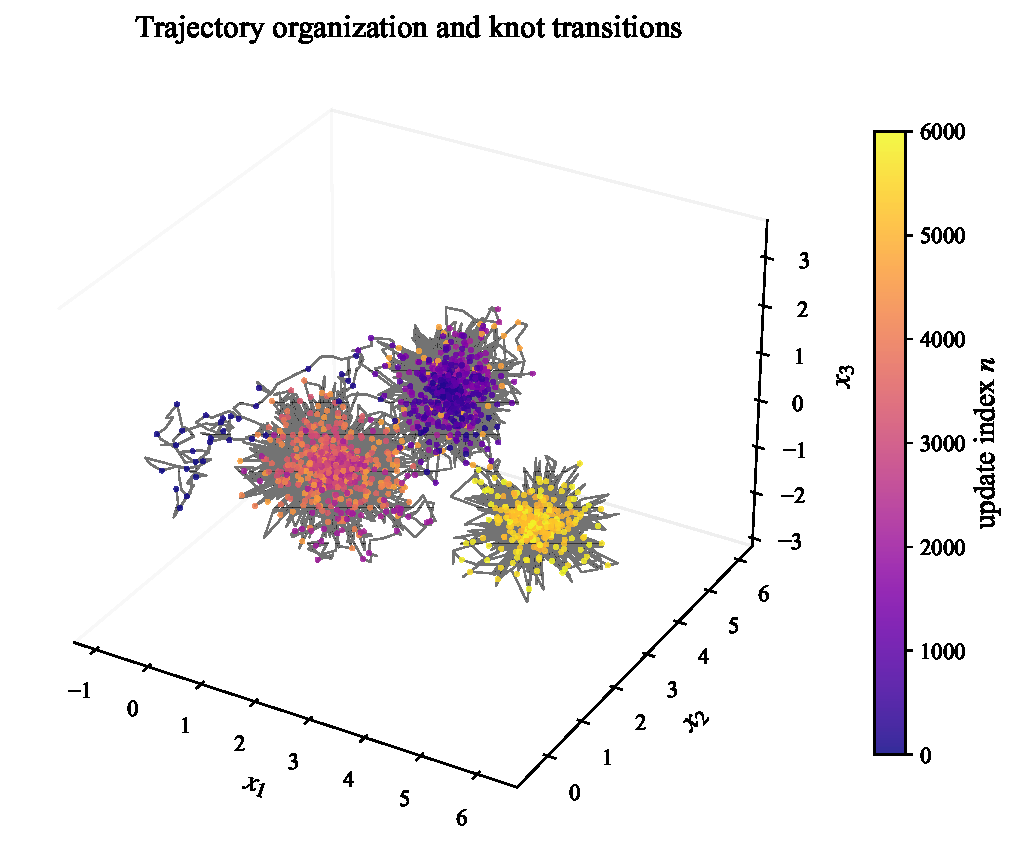
\includegraphics[width=0.88\linewidth]{fig3_knot_trajectory.pdf}
    \caption{
    Representative trajectory with multiple metastable knot-like regions.
    The line shows the visible trajectory, sampled points contribute to the memory density, and color denotes update index.
    }
    \label{fig:compact_knot_trajectory}
\end{figure}

A knot can be identified operationally by a region $\mathcal K\subset\Omega$ whose memory/visitation weight
\begin{equation}\label{eq:compact_memory_mass}
M_n(\mathcal K)=\int_{\mathcal K}\rho_n(x)\,dx
\end{equation}
remains elevated over intervals $\Delta n\gg\alpha^{-1}$.
Elevated $M_n(\mathcal K)$ means that the memory density carries substantial weight near $\mathcal K$; through Eq.~(\ref{eq:compact_potential}) this can generate a locally restoring drift that stabilizes the region against stochastic excursions.

In a frozen-memory approximation, knots can be represented locally by points or regions where
\begin{equation}
\nabla\Phi[\rho](x_\star)=0.
\end{equation}
Linearizing the continuum drift near such a point yields an OU-type approximation
\begin{equation}\label{eq:compact_ou}
\mathrm{d}x=-\gamma H(x-x_\star)\,\mathrm{d}t+\sqrt{2D}\,\mathrm{d}W_t,
\qquad
\gamma=\frac{\eta}{\alpha},
\end{equation}
where $H$ is the Hessian of the memory potential at $x_\star$.
Local stability requires the symmetric part of $H$ to be positive in the relevant directions \cite{Strogatz2018}.
If $\lambda$ denotes a characteristic restoring eigenvalue, the relaxation rate scales as
\begin{equation}\label{eq:compact_gamma_scale}
\Gamma_{\mathrm{rel}}\sim\frac{\eta}{\alpha}\lambda .
\end{equation}

\section{Relaxation Diagnostics}

The stability of a dynamical knot is measured by how quickly perturbations relax back into the metastable region.
Rare transitions are expected in the usual metastable regime of noisy dynamics \cite{Kramers1940,FreidlinWentzell2012}.
Let $\tau_{\mathrm{rel}}$ be extracted, for example, from an in-knot autocorrelation $C(t)\propto e^{-t/\tau_{\mathrm{rel}}}$ or from the dominant relaxation eigenvalue of the linearized Fokker--Planck operator.
We define
\begin{equation}\label{eq:compact_gamma}
\Gamma_{\mathrm{rel}}=\frac{1}{\tau_{\mathrm{rel}}}.
\end{equation}
Thus the diagnostic is a fitted decay scale of a coarse-grained trajectory observable, not a new microscopic parameter.

Because absolute coordinate scales on $\Omega$ are not physically fixed, it is useful to report the dimensionless combination
\begin{equation}\label{eq:compact_hat_gamma}
\widehat{\Gamma}=\frac{\sigma^2}{D}\Gamma_{\mathrm{rel}}.
\end{equation}
This compares relaxation to diffusion on the coarse-graining scale and is approximately invariant under uniform coordinate rescalings $x\mapsto ax$ with $\sigma\mapsto a\sigma$.
A second useful coarse-grained scale is
\begin{equation}\label{eq:compact_qrel}
Q_{\mathrm{rel}}=2D\Gamma_{\mathrm{rel}},
\end{equation}
which summarizes stochastic broadening and relaxation without assigning physical energy units.
A later calibration may determine whether a normalized version of this quantity can be interpreted as energy-like.

In this operational sense, a mass-like proxy is associated with relaxation or confinement strength rather than with a fundamental inertial parameter.
Heavier structures correspond to faster return to the metastable region and/or steeper memory-induced restoring potentials.
This terminology is only an effective-description shorthand; no identification with $mc^2$ or a relativistic mass scale is assumed here.

\section{Discussion}

We have introduced a minimal stochastic dynamics in which a visible point-valued state is coupled to an explicitly relaxing memory density.
The visible dynamics is generally non-Markovian, while the augmented state $(x_n,\rho_n)$ gives a natural Markov embedding.
The same memory update compresses ordered histories and therefore supplies an intrinsic update direction.
Coarse-graining on the memory-persistence scale yields the dimensionless parameter $t=\alpha n$ and, in suitable regimes, an approximate SDE/Fokker--Planck description.

Within this effective description, memory feedback can generate metastable dynamical knots.
Their stability can be characterized by residence weights, relaxation rates, and dimensionless diagnostics such as $\widehat{\Gamma}$.
These quantities are extractable from simulation trajectories and do not require physical spacetime units.

The construction remains intentionally limited.
The continuum SDE is an effective approximation rather than a proven scaling theorem, and the existence and classification of knot regimes depend on the qualitative properties of $(G_\sigma,K)$.
Multiple coupled generators, emergent geometry, universal constants, quantum normal forms, and Standard-Model-like structures are natural next questions, but they are not assumptions or conclusions of the present minimal model.

\begin{acknowledgments}
The author thanks colleagues for valuable feedback and discussion.
\end{acknowledgments}

\bibliographystyle{unsrtnat}
\bibliography{references}

\end{document}
